\documentclass[border=4pt]{standalone}
\usepackage{tikz}
\begin{document}

\noindent
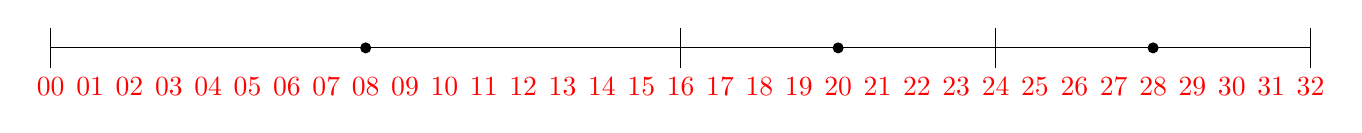
\begin{tikzpicture}[x=0.5cm,y=0.5cm]
  \draw (0.0,0.0) -- (32.0,0.0);
  \draw (0.0,-0.5) -- (0.0,0.5);
  \draw (32.0,-0.5) -- (32.0,0.5);
  \draw (16.0,-0.5) -- (16.0,0.5);
  \draw (24.0,-0.5) -- (24.0,0.5);
  \fill (8,0) circle(2pt);
  \fill (20,0) circle(2pt);
  \fill (28,0) circle(2pt);
  \foreach \x in {00,01,02,03,04,05,06,07,08,09,...,32} {
    \node (\x) at (\x,-0.5) [red,below]  {$\x$};
  }
\end{tikzpicture}

%% \noindent
%% \begin{tikzpicture}[x=0.5cm,y=0.5cm]
%%   \draw (0.0,0.0) -- (32.0,0.0);
%%   \draw (0.0,-0.5) -- (0.0,0.5);
%%   \draw (32.0,-0.5) -- (32.0,0.5);
%%   \draw (16.0,-0.5) -- (16.0,0.5);
%%   \draw (20.0,-0.5) -- (20.0,0.5);
%%   \draw (24.0,-0.5) -- (24.0,0.5);
%%   \fill (8,0) circle(2pt);
%%   \fill (18,0) circle(2pt);
%%   \fill (22,0) circle(2pt);
%%   \fill (28,0) circle(2pt);
%%   \foreach \x in {00,01,02,03,04,05,06,07,08,09,...,32} {
%%     \node (\x) at (\x,-0.5) [red,below]  {$\x$};
%%   }
%% \end{tikzpicture}

%% \noindent
%% \begin{tikzpicture}[x=0.5cm,y=0.5cm]
%%   \draw (0.0,0.0) -- (32.0,0.0);
%%   \draw (0.0,-0.5) -- (0.0,0.5);
%%   \draw (32.0,-0.5) -- (32.0,0.5);
%%   \draw (16.0,-0.5) -- (16.0,0.5);
%%   \draw (20.0,-0.5) -- (20.0,0.5);
%%   \draw (22.0,-0.5) -- (22.0,0.5);
%%   \draw (24.0,-0.5) -- (24.0,0.5);
%%   \fill (8,0) circle(2pt);
%%   \fill (18,0) circle(2pt);
%%   \fill (21,0) circle(2pt);
%%   \fill (23,0) circle(2pt);
%%   \fill (28,0) circle(2pt);
%%   \foreach \x in {00,01,02,03,04,05,06,07,08,09,...,32} {
%%     \node (\x) at (\x,-0.5) [red,below]  {$\x$};
%%   }
%% \end{tikzpicture}

%% \noindent
%% \begin{tikzpicture}[x=0.5cm,y=0.5cm,text centered]
%%   \node[align=center] {16\\$[0, 1]$}
%%     child {node[align=center] {08\\$[0, \frac{1}{2}]$}}
%%     child {node[align=center] {24\\$[\frac{1}{2}, 1]$}
%%       child {node[align=center] {20\\$[\frac{1}{2}, \frac{3}{4}]$}
%%         child {node[align=center] {18\\$[\frac{1}{2}, \frac{5}{8}]$}}
%%         child {node[align=center] {22\\$[\frac{5}{8}, \frac{3}{4}]$}
%%           child {node[align=center] {21\\$[\frac{5}{8}, \frac{11}{16}]$}}
%%           child {node[align=center] {23\\$[\frac{11}{16}, \frac{3}{4}]$}}
%%         }
%%       }
%%       child {node[align=center] {28\\$[\frac{3}{4}, 1]$}}
%%     };
%% \end{tikzpicture}

\end{document}


